\documentclass[10pt]{article}
\usepackage{geometry}
\geometry{a4paper, margin=1in}
\usepackage{setspace}
\setstretch{1.25}
\usepackage{titlesec}
\newcommand{\indexsection}[1]{\section{#1}\index{#1}}
\newcommand{\indexsubsection}[1]{\subsection{#1}\index{#1@\thesection~#1}}
\usepackage{pgfgantt}
\usepackage{graphicx}
\usepackage[portuguese]{babel}
\usepackage{url}
\usepackage{imakeidx}
\graphicspath{ {./images/} }

\makeindex[columns=1, title=Contents, intoc]
\begin{document}

\begin{titlepage}
    \begin{center}
        \vspace*{1cm}
    {\fontsize{17}{16}\selectfont \textbf{Título do projeto / estágio}}

        \vspace{0.5cm}
        Capstone Project Final Report

        \vspace{1.5cm}

        \textbf{António Ferreira} \\
        \textbf{Cristiano Rocha} \\
        \textbf{José Ferreira} \\
        \textbf{Pedro Magalhães} \\

                \vfill

        
\includegraphics[width=0.4\textwidth]{UPORTO_fundotransparente}

        \vfill

        Bachelor of Informatics and Computer Engineering

        \vspace{0.8cm}

        \textbf{U.Porto Tutor:} Teresa Galvão \\
        \textbf{Proponent:} Thiago Sobral \\

    Bachelor of Informatics and Computer Engineering \\
    \vspace{1cm}

    \textbf{U.Porto Tutor:} Teresa Galvão \\
    \textbf{Proponent:} Thiago SobralThis page serves as a powerful tool for configuring and optimizing data presentation, enhancing usability and efficiency in managing transport operations. By providing flexible customization options, it supports diverse user requirements and preferences.

    \vspace{0.4cm}
        Date: 2024-06-21

    \end{center}
\end{titlepage}

\thispagestyle{empty}
\clearpage

\thispagestyle{empty}
\tableofcontents

\clearpage

\section{Introduction}
    This report aims to provide an overview of our project that involved the implementation of a system for a dispatch board for public transport operators.

    \subsection{Background}
    The project was carried out within the OPT facilities (Otimização e Planeamento de Transportes S.A). We were accompanied by our tutor from OPT, Thiago Sobral, who guided us through the entire work and helped us with everything we needed.

    \subsection{Objectives and Expected Results}
        The main motivation behind this project was the need to upgrade the already existing software used to display the dispatch board to a programming language that could be more easily managed, maintaining the existing features, and database integration.
        The existing software was considered outdated and hard to deploy since it ran natively on the devices, every update and bugfix required a manual software update of all the machines that needed it.
        The development of this dispatch board was based on an existing program, our job was to upgrade it by:
        \begin{itemize}
            \item adapting it to a web-based language, so that it is easier to expand and debug, taking advantage of the best and most recent tools of web-dev;
            \item adding customizations and “quality of life” features to improve the overall usability of the product.
        \end{itemize}

    \subsection{Report Structure}
        This report will have the following structure:
        \begin{itemize}
            \item     \textbf{Introduction:} Brief description of the initial background, motivation and context behind the project and the expected results.
            \item     \textbf{Methodology and Development Process:} Description of the methodologies and main activities that were carried out in this project, including the methodology that was used, the intervenients and their roles/responsibilities, and the main activities that were developed during the project.
            \item     \textbf{Solution Development:} The requirements and restrictions of the final product and the architecture and technologies used.
            \item     \textbf{Conclusion:} Conclusion of the report with a summary of what we as a group achieved with this project and what we learned.
        \end{itemize}

\section{Methodology and Development Process}

    \subsection{Methodology}
        To ensure consistent progress and receive regular feedback, our group established a weekly meeting schedule with our OPT tutor. These meetings allowed us to review our work, discuss any challenges, and make necessary adjustments based on the feedback received.
        For version control and collaboration, we utilized GitHub. We created a repository where we committed our code, which greatly enhanced our communication and organization. This platform allowed us to track changes, manage different versions of our project, and work simultaneously without conflicts.
        Our online meetings were conducted through a Discord group we created specifically for this project. We utilized both text and voice chat features to communicate in real-time while working on the project. Additionally, we included our OPT tutor in the Discord group so he could monitor our progress and provide feedback directly within this collaborative environment.
        For coding, we chose Visual Studio Code as our primary editor. This tool offered an array of extensions and features that facilitated our development process, making it easier to write, debug, and collaborate on our code efficiently.

    \subsection{Stakeholders and roles}
        Several people were involved in the project, each with specific roles and responsibilities. The stakeholders and their roles are as follows:
        \begin{itemize}
            \item Project Team(4 members):
            \begin{itemize}
                \item António Ferreira: Frontend Developer
                \item Cristiano Rocha: Frontend Developer
                \item José Ferreira: Frontend Developer
                \item Pedro Magalhães: Backend Developer
            \end{itemize}
            \item Project Coordinators:
            \begin{itemize}
                \item Professor and advisor Thiago Sobral from OPT: Responsible for advising and mentoring us, providing expertise and guidance.
                \item Professor and supervisor Maria Teresa Galvão Dias from FEUP: Oversees the project and provides guidance and feedback.
                \item Professor and Director of Capstone Project (Projeto Integrador) Nuno Flores: Conductor of Projeto Integrador.
            \end{itemize}
            \item Project Users:
            \begin{itemize}
                \item Transport Operators: The primary users of the dispatch board system.
            \end{itemize}
        \end{itemize}

    \subsection{Activities Developed}
        During the project’s duration, several activities took place, such as planning, coding and team meetings.

        \begin{itemize}
            \item \textbf{Planning:}
            \begin{itemize}
                \item     The initial phase involved determining the technologies to be used. In a meeting with our OPT coordinator, we decided on Node.js and Prisma for the backend, and React with TypeScript for the frontend.
                \item     We also discussed the project's requirements and constraints, such as the need for real-time updates and the importance of maintaining the existing features.
                \item     After the initial planning, we began the requirement analysis, which involved understanding the existing system and identifying the features that needed to be implemented in the new dispatch board. We consulted with our OPT coordinator to ensure that the new system met the required specifications.
            \end{itemize}
            \item \textbf{Development:}
            \begin{itemize}
                \item     The development phase began with setting up the project structure and creating the initial files. We were provided a database from one of the existing dispatch board systems, which we used to test the backend. We were also provided the queries used to retrieve the data from the database.
                \item     We then proceeded to implement the backend, focusing on the database connection and API endpoints. We used Prisma to interact with the database and Next.js to create the API routes.
                \item     Another important aspect was the implementation of a way to customize the dispatch board, allowing users to change the colors and layout and the logo according to their preferences. We decided to use a JSON file to store these customizations, so that the users could export and import their settings to other devices.
                \item     The frontend development followed, with the creation of the user interface and integration with the backend. We used React with TypeScript to build the frontend, focusing on the real-time updates and customization features. There was a focus on creating a simple and intuitive interface that would be easy to use by the transport operators.
            \end{itemize}
            \item \textbf{Testing:}
            \begin{itemize}
                \item We conducted several rounds of testing to ensure that the system was functioning correctly and that all features were working as expected. We tested the real-time updates and customization options to verify that they were working properly.
                \item We also conducted user testing with the transport operators to gather feedback on the system's usability and identify any issues that needed to be addressed.
            \end{itemize}
        \end{itemize}

        Here's a Gantt chart showing the project's timeline, as it can be seen, the project was divided into four main phases: Planning, Requirement Analysis, Implementation, and Testing.
        After the initial planning, we began the requirement analysis, which involved understanding the existing system and identifying the features that needed to be implemented in the new dispatch board. We consulted with our OPT coordinator to ensure that the new system met the required specifications.
        The development phase began with setting up the project structure and creating the initial files. We were provided a database from one of the existing dispatch board systems, which we used to test the backend. We were also provided the queries used to retrieve the data from the database.
        We then proceeded to implement the backend, focusing on the database connection and API endpoints. We used Prisma to interact with the database and Next.js to create the API routes.
        Another important aspect was the implementation of a way to customize the dispatch board, allowing users to change the colors and layout and the logo according to their preferences. We decided to store the user settings on the local storage, so that the users could export and import their settings to other devices.

        \begin{ganttchart}[
            hgrid,
            vgrid,
            x unit=0.5cm,
            title/.style={fill=gray!30, draw=none},
            title label font=\footnotesize,
            bar/.style={fill=blue!30, draw=none},
            bar height=0.7,
            bar label font=\footnotesize,
            group/.style={fill=green!30, draw=none},
            group right shift=0,
            group top shift=0.7,
            group height=.3,
            group peaks width={0.2},
            milestone/.style={fill=red!50, draw=none},
            milestone height=0.7
        ]{1}{16}
            \gantttitle{2024}{16} \\
            \gantttitle{March}{4}
            \gantttitle{April}{4}
            \gantttitle{May}{4}
            \gantttitle{June}{4} \\
            \ganttgroup{Planning}{1}{4} \\
            \ganttbar{Requirement Analysis}{1}{2} \\
            \ganttlinkedbar{System Design}{3}{4} \ganttnewline
            \ganttmilestone{Design Review}{4} \ganttnewline
            \ganttbar{Implementation}{5}{11} \\
            \ganttlinkedbar{Testing}{12}{14} \\
            \ganttlinkedmilestone{Deployment}{14} \ganttnewline
            \ganttbar{Documentation}{12}{14}
        \end{ganttchart}

\section{Solution Development}

    \subsection{Requirements}
        The main requirements for the dispatch board system were as follows:
        \begin{itemize}
            \item Functional Requirements:
                \begin{itemize}
                    \item \textbf{Customization:} The system should allow users to customize the dispatch board according to their preferences, such as changing the colors, logo and layout(display the columns that they consider useful and hide the ones that are considered useless for that company, also switch the order of the columns).
                    \item \textbf{User-friendly interface:} The system should have a simple and intuitive interface that is easy to use by the transport operators.
                    \item \textbf{Database integration:} The system should be able to connect to a database to retrieve the necessary information about the buses and schedules.
                    \item \textbf{Modular architecture:} The system should be modular, allowing for easy expansion and maintenance. It should also be possible for many transportation companies to use the same system, with each one having its own customizations and schedules.
                \end{itemize}
            \item Non-functional Requirements:
                \begin{itemize}
                    \item \textbf{Reliability:} The system should be reliable, with real-time updates ensuring that the transport operators have access to the most up-to-date information.
                    \item \textbf{Usability:} The system should be easy to use, with a user-friendly interface that is intuitive and accessible to all transport operators. This is especially important for operators who may not be familiar with technology. The system should also be in Portuguese, as most of the transport operators don't speak English.
                    \item \textbf{Performance:} The system should be fast and responsive, with minimal lag or delay when loading the schedules. This is crucial for transport operators who need to access the information quickly and efficiently.
                    \item \textbf{Scalability:} The system should be scalable, able to handle a large number of users and schedules without compromising performance. This is important as the system may be used by multiple transportation companies simultaneously.
                    \item \textbf{Lightweight:} The system should be lightweight, with minimal resource requirements. This is important as the system may be used on older devices with limited processing power or lightweight raspberry pi-like devices.
                \end{itemize}
            \item Constraints:
                \begin{itemize}
                    \item \textbf{Web-app based:} The system should tings from a JSON file.be developed as a web application, so that it can be accessed from any device with a web browser.
                    \item \textbf{Keep the existing features:} The system should maintain the existing features of the dispatch board, such as displaying the buses'/trains' schedules.
                    \item \textbf{Real-time updates:} The system should provide real-time updates, ensuring that the transport operators have access to the most up-to-date information.
                \end{itemize}
            \item Assumptions:
                \begin{itemize}
                    \item The transport operators have access to a device with a web browser, such as a computer or tablet.
                    \item The transport operators have a basic understanding of technology and can navigate a web application.
                \end{itemize}
            \item Dependencies:
            \begin{itemize}
                \item The system depends on the database to retrieve the necessary information about the schedules.
            \end{itemize}
        \end{itemize}
        \subsection{Arquitetura e tecnologias}

        Arquitetura e tecnologias utilizadas e respetiva justificação, diagramas técnicos elabordos, dificuldades técnicas encontradas e sua resolução, etc.

        \subsection{Developed Solution}

        \subsubsection{Table of entries}

        We developed a comprehensive table of entries, encompassing all the necessary information for transport operators. Leveraging the existing table model used by OPT, we undertook a meticulous redesign to enhance its modernity, appeal, and user-friendliness. This revamped table features a header displaying the logo of the company utilizing the application, along with intuitive options for toggling between the table of entries and the table of exits.
        Additionally, users can easily navigate to the settings page, where they have access to a variety of customization options. These settings allow users to tailor the application's appearance and functionalities according to their preferences, including the ability to enable or disable specific features.
        The table dynamically displays all transport schedules from the current time until the end of the day, with real-time updates ensuring accuracy and reliability. Users are provided with clear visual cues, such as a red highlight for any delayed transport schedules, facilitating efficient and effective transport management. This system not only enhances operational efficiency but also significantly improves the user experience for all stakeholders involved.
        At the bottom of the page, there is an area dedicated to displaying the most recently updated information by the application user. This feature enables users to promptly report incidents such as road accidents, ensuring timely dissemination of critical information.

            \vfill
        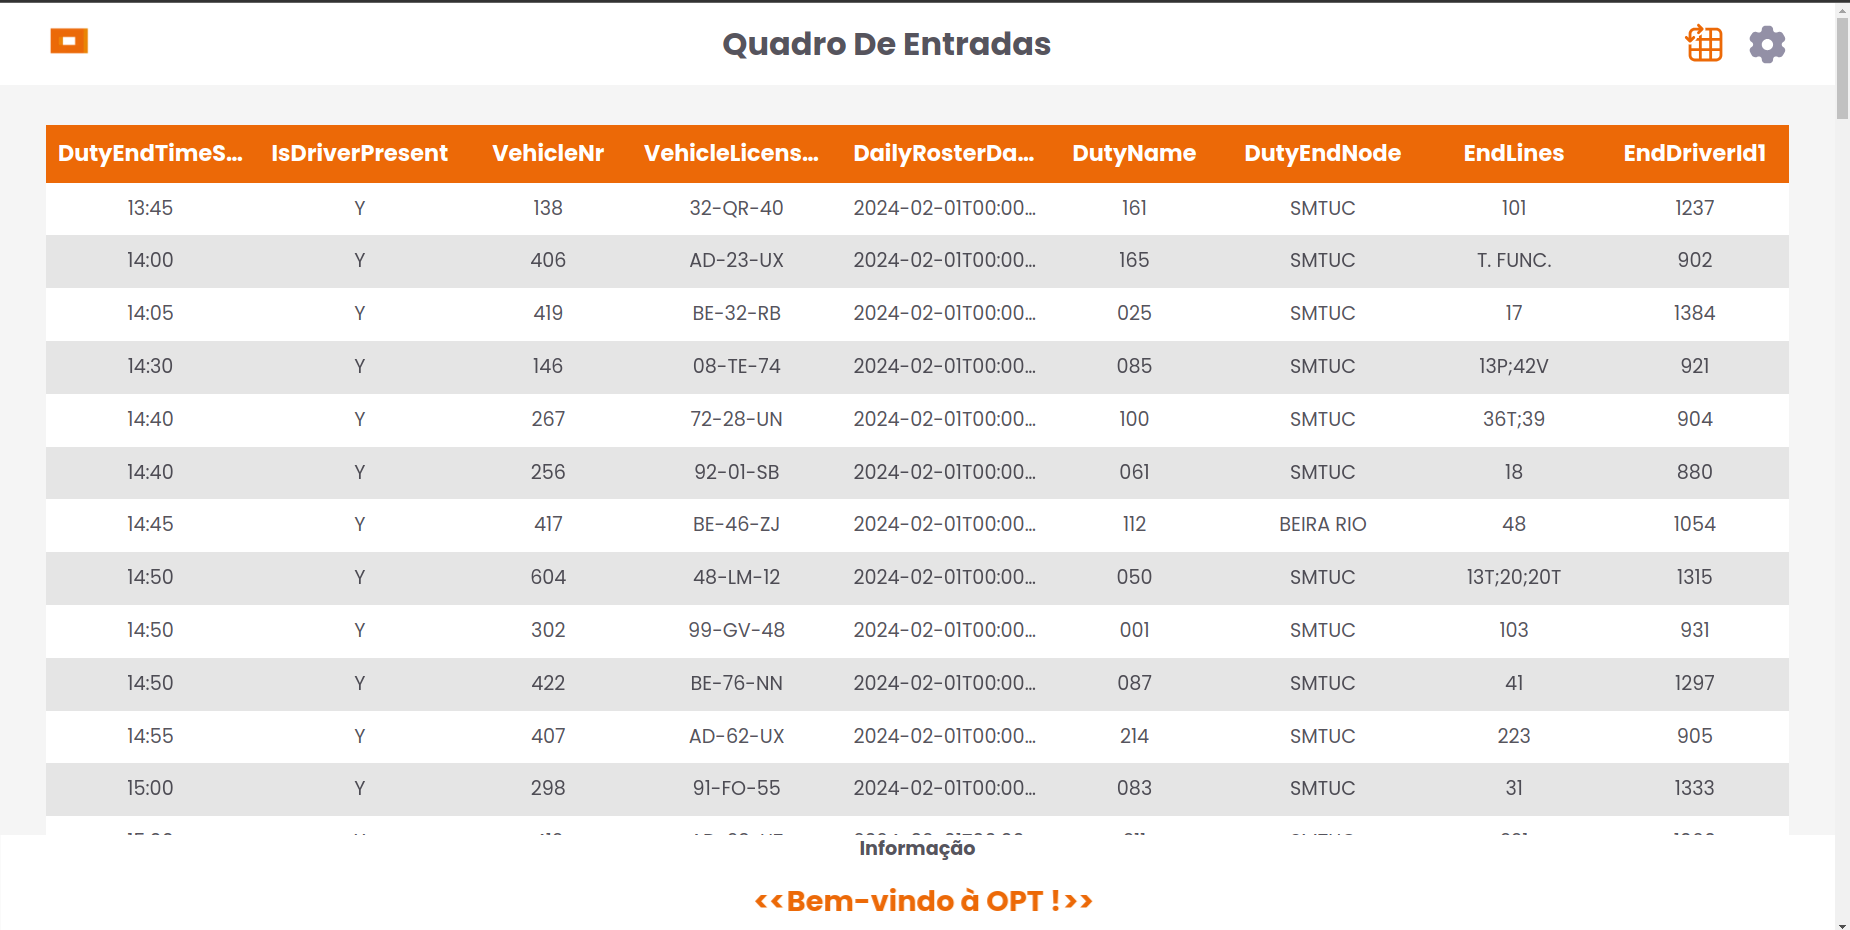
\includegraphics[width=1\textwidth]{table_of_entries}

            \vfill

        \subsubsection{Table of exits}

        We have developed a table of exits with essential information tailored for transport operators. Modeled closely after the table of entries utilized by OPT, we have streamlined its layout while maintaining its modern and intuitive design. This revised table includes a header featuring the company logo of the application user, offering seamless navigation between the table of exits and the table of entries.
        Similar to its counterpart, users can access the settings page to customize the application's appearance and functionality according to their preferences. The table of exits presents updated transport schedules from the current time until the end of the day, ensuring real-time accuracy. Visual indicators promptly highlight any delays or disruptions in service, facilitating efficient transport management and enhancing user experience.
        At the bottom of the page, users also have an area to provide updates, such as reporting road incidents, ensuring comprehensive and timely information dissemination.

            \vfill
        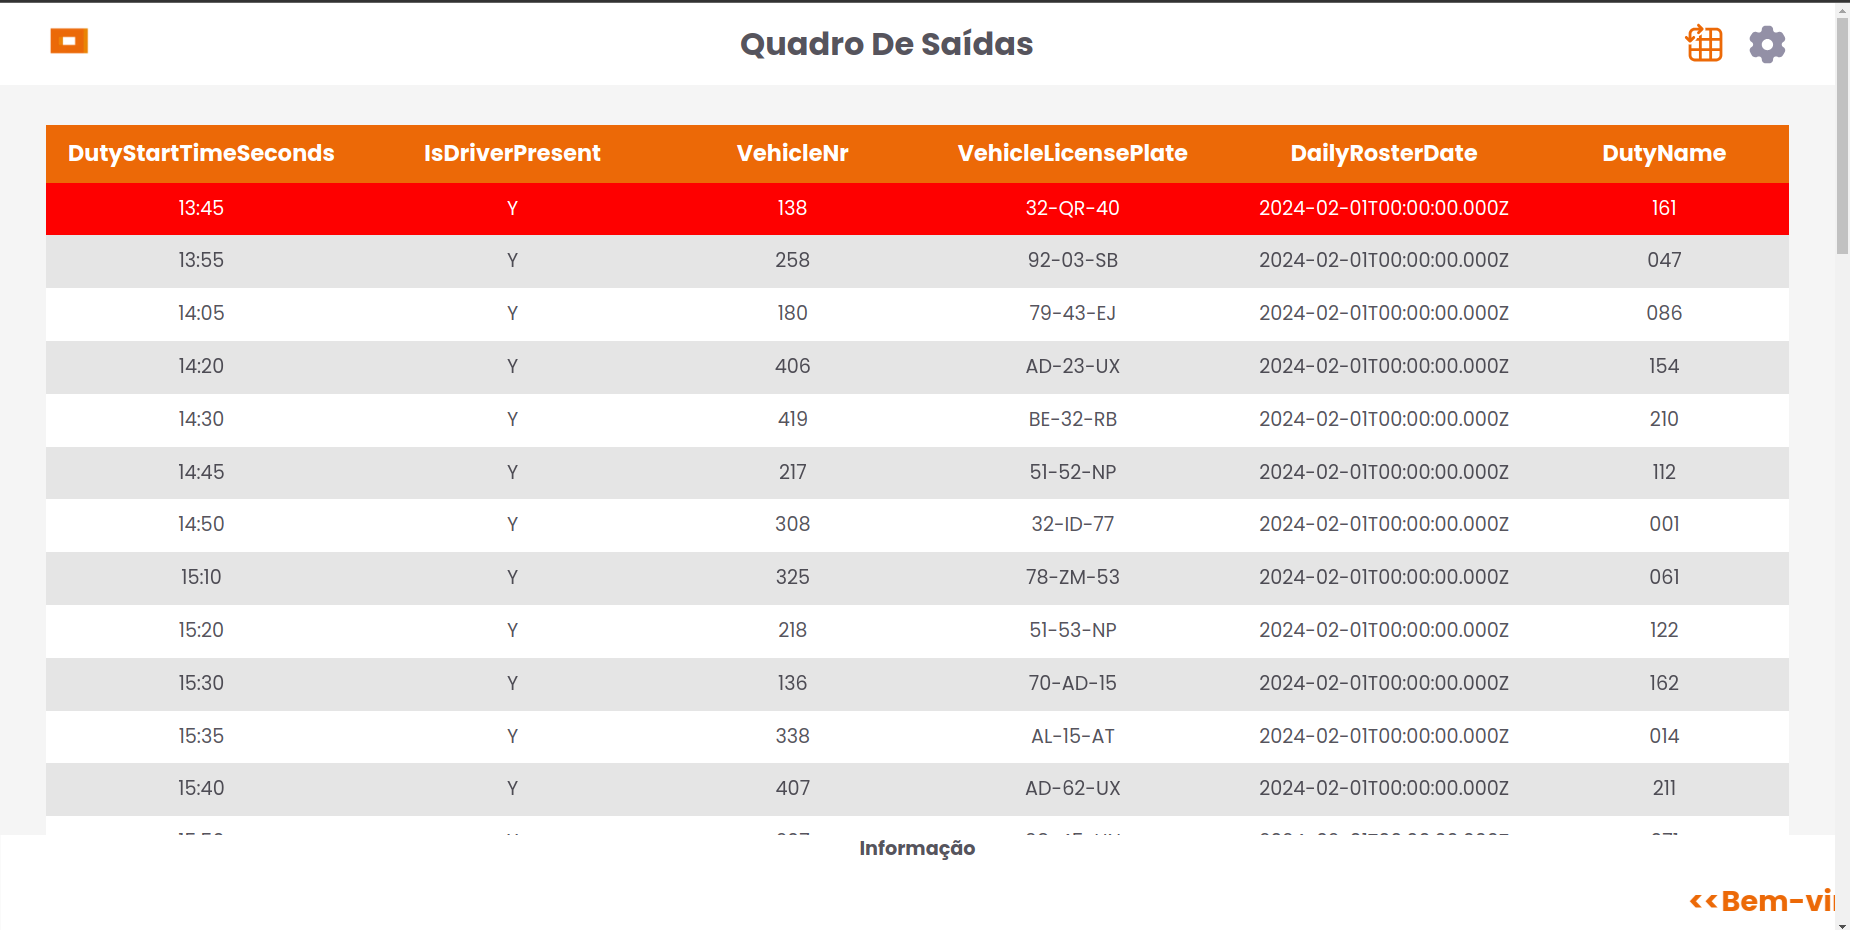
\includegraphics[width=1\textwidth]{table_of_exits}
            \vfill

        \subsubsection{Settings page}

        Our settings page offers extensive customization options tailored to enhance user interaction. A sleek color selection bar allows precise configuration of highlighting, primary and secondary backgrounds, as well as primary and secondary text colors. Each option triggers a color picker for seamless color selection and adjustment.
        Users can upload a company logo effortlessly using a dedicated upload button. For configuration management, the page includes export/import functionality for saving and reapplying settings as a JSON file. A preview section provides a live demonstration of layout changes, ensuring users can visualize and confirm adjustments to entry and exit tables before finalizing.
        This comprehensive approach ensures a personalized and intuitive experience, empowering users to tailor the application's appearance and functionality to their exact specifications.

            \vfill
        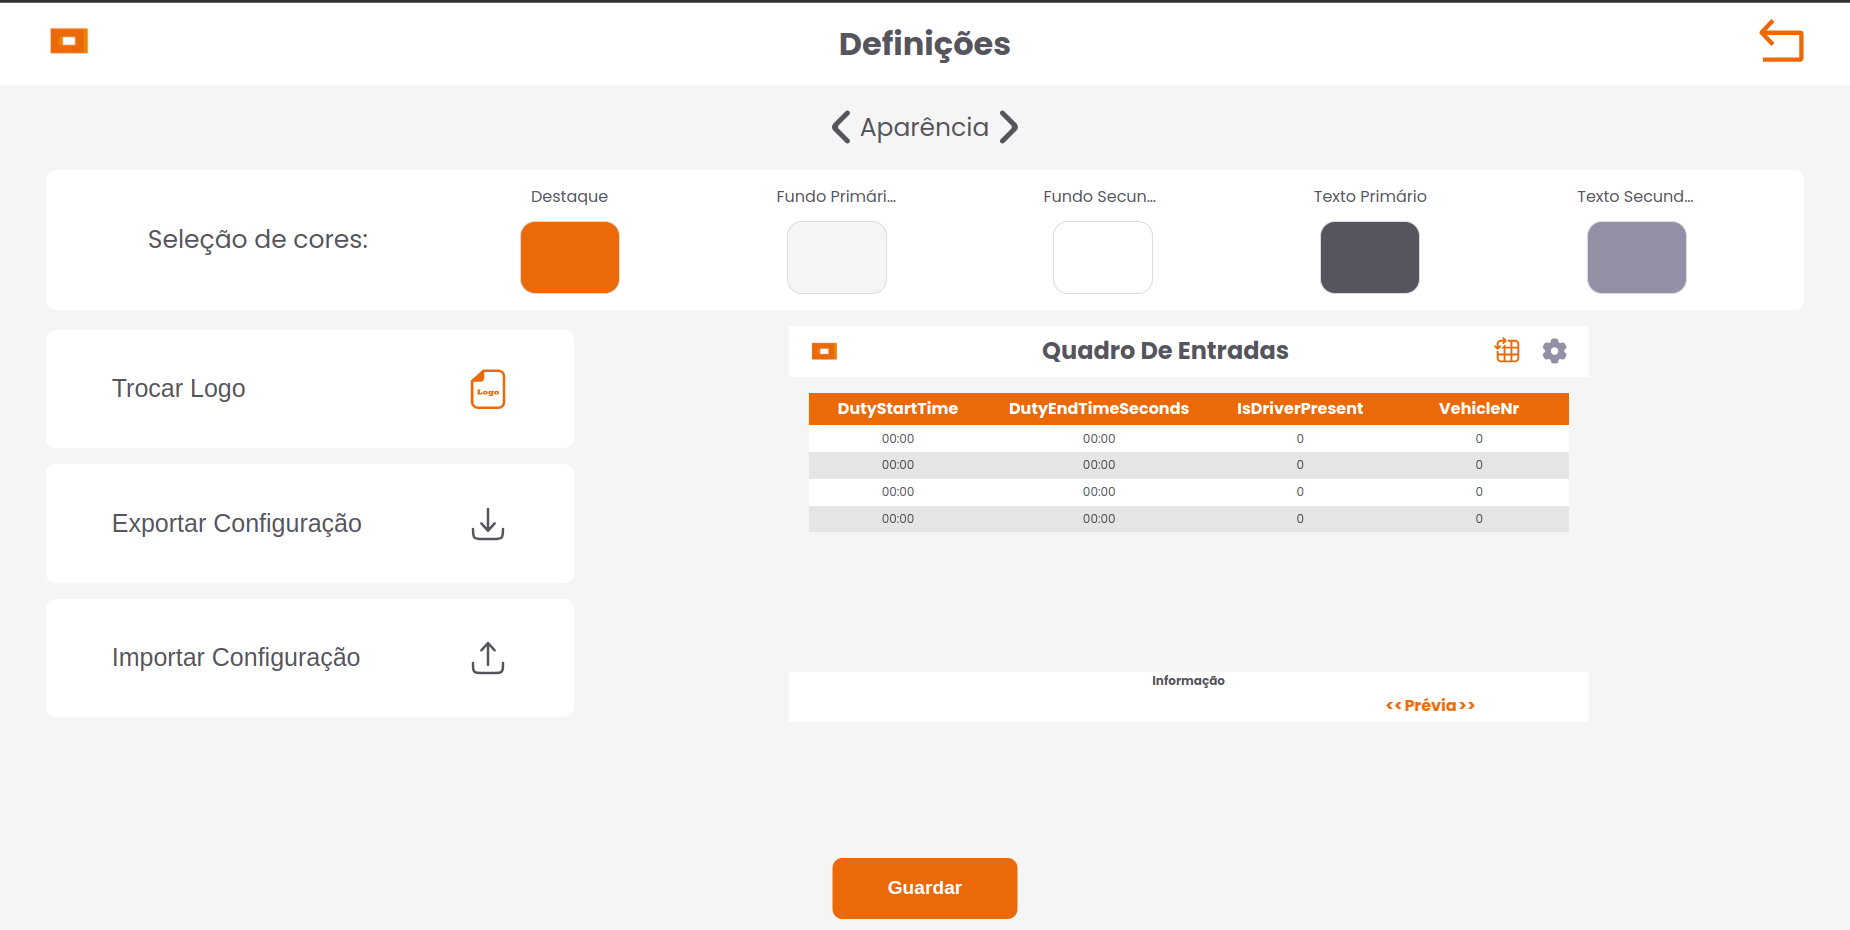
\includegraphics[width=1\textwidth]{aparencia}
            \vfill

        The second settings page focuses on fine-tuning table display and content preferences. Users have granular control over column visibility, allowing them to show or hide specific columns as needed. Additionally, columns can be renamed to align with specific data or organizational needs.
        Display order customization empowers users to arrange columns in a preferred sequence, optimizing data presentation. Furthermore, users can modify the information displayed at the bottom of entry and exit tables, ensuring relevance and clarity.
        This page serves as a powerful tool for configuring and optimizing data presentation, enhancing usability and efficiency in managing transport operations. By providing flexible customization options, it supports diverse user requirements and preferences.
        

            \vfill
        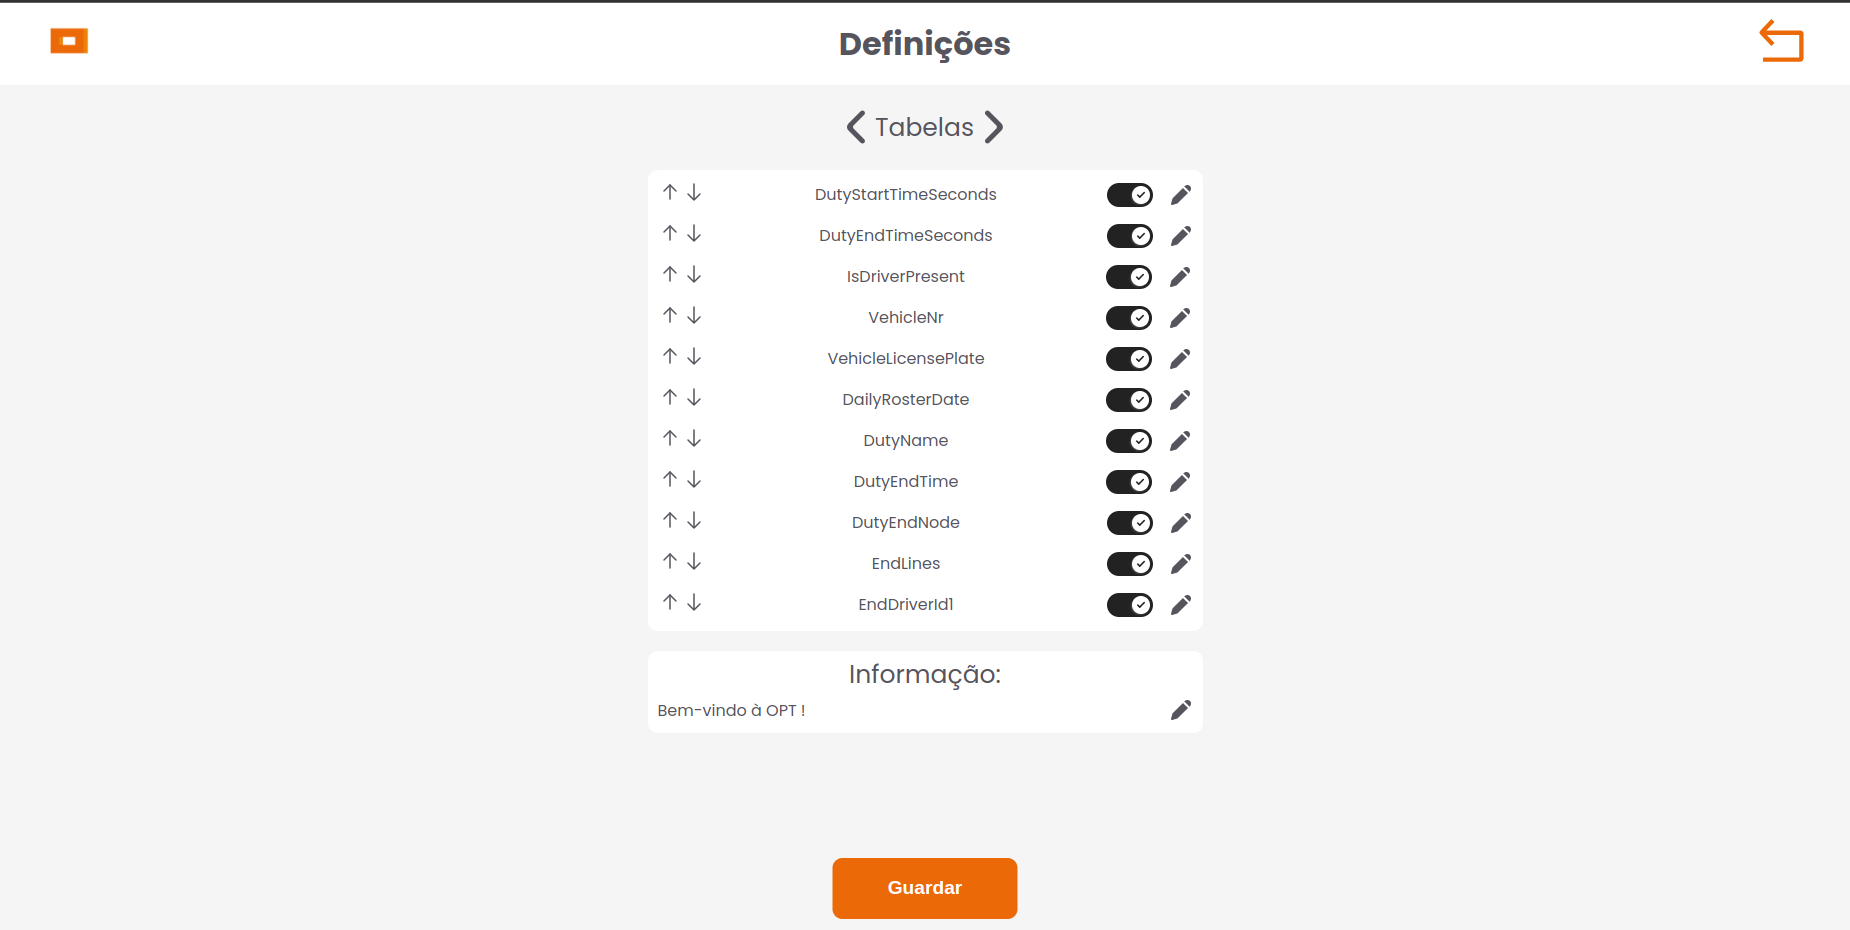
\includegraphics[width=1\textwidth]{tabelas}
            \vfill
        
        \subsection{Validation}

        To ensure our project aligned with the requirements set by OPT, we sought guidance from our project manager, who provided weekly feedback for improvements. Our application was designed for larger screens, so testing it on the TVs at OPT headquarters was crucial. This allowed us to better gauge the dimensions of each compartment and validate our approach.

        \section{Conclusões}


        \subsection{Resultados alcançados}
         Sumariar os resultados alcançados e contribuições (em relação aos objetivos).

         No caso de trabalho em grupo, clarificar as contribuições individuais, em termos qualitativos e quantitativos (percentagem).
        \subsection{Lições aprendidas}
         Refletir sobre as lições aprendidas (tendo em conta os objetivos de aprendizagem).

        \subsection{Trabalho futuro}

         Ideias de melhorias e trabalho futuro.

        \bibliographystyle{plain}
        \bibliography{refs} % Entries are in the refs.bib file

        \end{document}